\chapter{ヒッグス機構：ゲージボソンはいかにして質量を獲得するか}

ここで、前回の講義で展開した二つの考えを結び合わせる。大域的\(U(1)\)対称性が破れた複素スカラー場には、質量をもつ動径方向の振動と質量ゼロの角度方向の振動が含まれる。局所的に不変な\(U(1)\)理論には質量ゼロのゲージ場が含まれる。スカラーが電荷をもち、その平衡値の大きさがゼロでないとき、これらの主張を単純に足し合わせることはできない。角度方向のモードとゲージ場が結合する。すなわち、ゲージ場は質量をもつようになり、見かけのゴールドストーンボソンは独立な粒子ではなくなり、動径方向のヒッグスモードが残る。

光子を模型的なゲージボソンとして用いるが、それが物理的な結論ではない。電磁\(U(1)\)は真空中で破れていないので、実光子は質量ゼロである。同じ機構は電弱理論において\(W^\pm\)と\(Z\)に働くが、そこではゲージ群とスカラー多重項がより複雑である。アーベル模型は、群論の下に機構を隠すことなく、その機構を露わにする。

\begin{classroomqa}
\audiencequestion{これまでの議論は、ヒッグス機構が実光子に質量を与えるという意味だったのか。\lecturetimestamp{00:00:23}}
\lecturerresponse{いいえ。光子に対応する\(U(1)\)が破れた相にあると\emph{仮に}したら何が起こるかを問うているのである。その仮想的な光子は質量をもつようになるだろう。実際の電磁真空はその相にはなく、素粒子物理学への応用は代わりに\(W\)と\(Z\)の質量である。}
\end{classroomqa}

電荷の保存に対応する対称性は、位相回転
\begin{equation}
  \phi(x)\longmapsto e^{i\theta}\phi(x),
\end{equation}
であり、\(U(1)\)と呼ばれる内部回転である。超伝導体は、破れた相の実在する類似物を与える。その内部では、電磁場は有限の侵入長をもち、重要な点で質量をもつ場のように振る舞う。その外部では、通常の質量ゼロの光子が再び現れる。

\section{場にとって質量とは何を意味するか}

\subsection{分散関係とゼロ運動量ギャップ}

ヒッグス場を導入する前に、質量によって何を意味するのかを正確に定めておく価値がある。波に対しては
\begin{equation}
  E=\hbar\omega,
  \qquad
  p=\hbar k,
  \label{eq:l08-quantum-wave}
\end{equation}
であるから、\((E,p)\)のグラフと\((\omega,k)\)のグラフは、\(\hbar\)の因子を除いて同じ情報を含む。空の空間では、質量ゼロの相対論的励起は
\begin{equation}
  E=c|p|,
  \qquad
  \omega=c|k|.
  \label{eq:l08-massless-dispersion}
\end{equation}
に従う。\(k\)の二つの符号は、反対向きの伝播方向を区別する。本質的な点は、\(\omega\)が\(k\)とともにゼロに近づくことである。

質量をもつ相対論的粒子は
\begin{equation}
  E^2=c^2p^2+m^2c^4.
  \label{eq:l08-massive-dispersion}
\end{equation}
に従う。単位\(c=\hbar=1\)では、
\begin{equation}
  \omega^2=k^2+m^2.
\end{equation}
である。\(k=0\)において、エネルギーは\(E=mc^2\)、すなわち自然単位では単に\(m\)である。したがって質量とは、ゼロ運動量モードのゼロでないエネルギーギャップである。

\begin{figure}[htbp]
\centering
\begin{adjustbox}{max width=\linewidth}
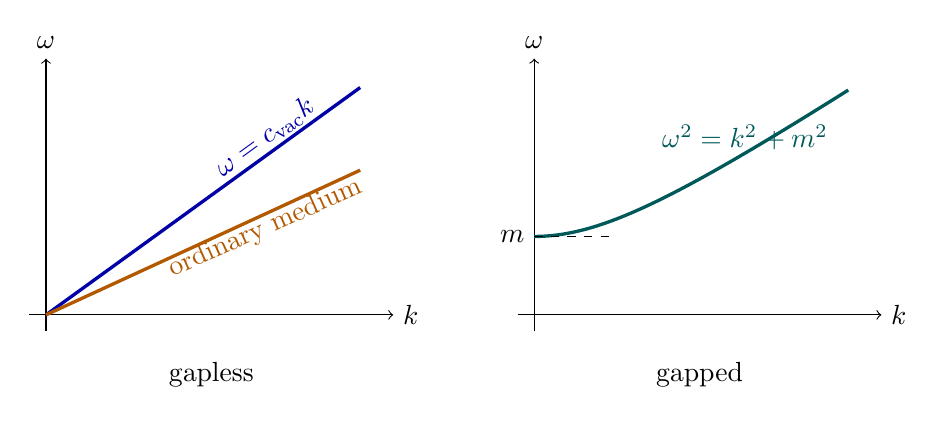
\begin{tikzpicture}[x=1.05cm,y=1.05cm]
  \begin{scope}
    \draw[->] (-0.2,0) -- (4.2,0) node[right] {\(k\)};
    \draw[->] (0,-0.2) -- (0,3.1) node[above] {\(\omega\)};
    \draw[very thick,blue!65!black] (0,0) -- (3.8,2.75);
    \draw[very thick,orange!70!black] (0,0) -- (3.8,1.75);
    \node[blue!65!black,rotate=36] at (2.65,2.15)
      {\(\omega=c_{\rm vac}k\)};
    \node[orange!70!black,rotate=24] at (2.65,1.05)
      {ordinary medium};
    \node[below] at (2,-0.45) {gapless};
  \end{scope}
  \begin{scope}[xshift=6.2cm]
    \draw[->] (-0.2,0) -- (4.2,0) node[right] {\(k\)};
    \draw[->] (0,-0.2) -- (0,3.1) node[above] {\(\omega\)};
    \draw[very thick,domain=0:3.8,samples=120,smooth,teal!70!black]
      plot (\x,{sqrt(0.9+0.45*\x*\x)});
    \draw[dashed] (0,0.95) -- (1.0,0.95);
    \node[left] at (0,0.95) {\(m\)};
    \node[teal!70!black] at (2.55,2.15)
      {\(\omega^2=k^2+m^2\)};
    \node[below] at (2,-0.45) {gapped};
  \end{scope}
\end{tikzpicture}
\end{adjustbox}
\caption{伝播速度を変えると、ギャップのない分散関係の傾きが変わる。励起に質量を与えると、\(k=0\)においてゼロでないギャップが開く。}
\label{fig:l08-dispersion}
\end{figure}

通常の透明な物質は、この相対論的な質量ギャップを生じさせることなく、波の位相速度を低下させうる。境界では、入射周波数は固定され、波数は媒質の分散関係に合わせて調整される。傾きを変えることは、切片を持ち上げることと同じではない。
\editorialnote{物質は複数の電磁分岐をもちうるし、プラズマや共鳴媒質はゼロでないプラズマ周波数ギャップをもちうる。本講義の比較は、特に通常の屈折分岐と超伝導応答の間のものである。より一般には、ギャップがないとは\(k\to0\)のとき\(\omega(k)\to0\)となることを意味し、すべての非相対論的媒質において厳密な線形性は要求されない。}

\begin{classroomqa}
\audiencequestion{光子は、たとえばプリズムを通る場合のように、物質中を進むときはいつでも質量を獲得するのか。\lecturetimestamp{00:03:02}}
\lecturerresponse{いいえ。屈折は周波数と波数の関係を変え、したがって伝播速度を変えうるが、その分岐は依然として\(k=0\)において\(\omega=0\)を通る。それに対して超伝導相は、電磁応答に有限の逆侵入長、すなわち質量の類似物を与える。}
\end{classroomqa}

\begin{classroomqa}
\audiencequestion{固定した周波数の光がガラスに入るとき、変化するのは波数のほうか。\lecturetimestamp{00:09:20}}
\lecturerresponse{はい。静止した界面における時間並進不変性が周波数を固定する。ガラス中では分散曲線の傾きが異なるので、同じ\(\omega\)は異なる\(k\)に対応し、したがって異なる波長に対応する。}
\end{classroomqa}

傾き
\begin{equation}
  v_g=\frac{d\omega}{dk}
\end{equation}
は波束の群速度である。その傾きが\(k\)とともに変化するなら、異なるフーリエ成分は異なる速度で進み、波束は分散する。これが、関係\(\omega(k)\)が\emph{分散関係}と呼ばれる理由である。

\begin{classroomqa}
\audiencequestion{この曲線の名前は何か、またその傾きは何を表すのか。\lecturetimestamp{00:11:02}}
\lecturerresponse{この曲線は分散関係である。その導関数
\(d\omega/dk\) は群速度である。傾きが一定ならすべての波長に同じ速度を与える。傾きが変化すれば波束は広がる。ここでの目的にとって決定的な区別は、曲線が原点に達するか、それともギャップをもつかである。}
\end{classroomqa}

\subsection{一様な振動は静止した粒子である}

モード \(k=0\) は無限の波長をもつ。すなわち場はどこでも同じだけ変位している。一様な変位を与えて放す。もし場が非零の振動数で振動するなら、対応する量子は非零の静止エネルギーをもち、質量をもつ。もしその方向に復元力がなければ、振動数は消え、そのモードは質量ゼロである。

この記述は古典的である。空間的に離れた粒子が量子重ね合わせにあることを必要としない。一様な古典場の配位とは、単に一つの場の値が空間全体で繰り返されているものにすぎない。

\begin{classroomqa}
\audiencequestion{場全体が一緒にずれることは、量子もつれと同じことか。\lecturetimestamp{00:10:04}}
\lecturerresponse{いいえ。一様な古典場は一つの古典的配位である。もつれは、上--下や下--上といった異なる量子選択肢を相関させる。同じ場の値を多くの点で用意することは、それ自体ではもつれではなく、瞬時の因果的応答を意味するものでもない。}
\end{classroomqa}

正準に規格化された実スカラー場に対して、
\begin{equation}
  \mathcal L
  =\frac12\partial_\mu\varphi\,\partial^\mu\varphi-V(\varphi),
\end{equation}
平衡値 \(\varphi_0\) のまわりで展開する：
\begin{equation}
  V(\varphi_0+\eta)
  =V(\varphi_0)
   +\frac12V''(\varphi_0)\eta^2+\cdots.
\end{equation}
線形項は最小値で消え、場の方程式は次を与える。
\begin{equation}
  \omega^2=\bm{k}^2+m^2,
  \qquad
  m^2=V''(\varphi_0).
  \label{eq:l08-curvature-mass}
\end{equation}
したがって質量は、運動の方向におけるポテンシャルの曲率である。平坦な方向は曲率ゼロであり、質量ゼロのモードを与える。

\section{破れた複素スカラー}

\subsection{動径運動と角度運動}

複素スカラーをデカルト座標と極座標で書く：
\begin{equation}
  \phi=\phi_R+i\phi_I=\rho e^{i\alpha},
  \qquad
  \phi^*=\phi_R-i\phi_I=\rho e^{-i\alpha}.
  \label{eq:l08-polar-field}
\end{equation}
複素平面は\emph{内部}場の空間である。各物理的時空点 \(x\) において、対
\((\phi_R(x),\phi_I(x))\) はその内部平面内の一点を指定する。どちらの内部軸も実験室の方向ではない。

\begin{figure}[htbp]
\centering
\includegraphics[width=0.72\textwidth]{lecture_08_figure_02.png}
\caption{内部\((\phi_R,\phi_I)\)平面で表された複素スカラー。半径は \(\rho\) であり、\(\alpha\) は内部位相である。}
\lectureframe{00:24:41}
\label{fig:l08-internal-plane}
\end{figure}

スカラーの運動項は次になる。
\begin{align}
  \partial_\mu\phi^*\,\partial^\mu\phi
  &=
  \partial_\mu\phi_R\,\partial^\mu\phi_R
  +\partial_\mu\phi_I\,\partial^\mu\phi_I
  \notag\\
  &=
  \partial_\mu\rho\,\partial^\mu\rho
  +\rho^2\partial_\mu\alpha\,\partial^\mu\alpha.
  \label{eq:l08-polar-kinetic}
\end{align}
大域的 \(U(1)\) 不変なポテンシャルは \(\phi^*\phi=\rho^2\) に依存し、\(\alpha\) には依存しない。例えば、
\begin{equation}
  V(\phi)
  =\lambda\left(\phi^*\phi-\frac{f^2}{2}\right)^2,
  \qquad \lambda>0.
  \label{eq:l08-mexican-hat}
\end{equation}
その最小値は円をなす。法則は共通の位相回転の下で不変であるが、一つの平衡位相を選ぶことは円上の一点を選ぶことになる。

\begin{figure}[htbp]
\centering
\includegraphics[width=0.78\textwidth]{lecture_08_figure_03.png}
\caption{板書の動径ポテンシャルのスケッチ。ポテンシャルは内部場の値の回転の下で対称であるが、場自体は原点に位置する必要はない。}
\lectureframe{00:34:22}
\label{fig:l08-radial-potential-board}
\end{figure}

\begin{figure}[htbp]
\centering
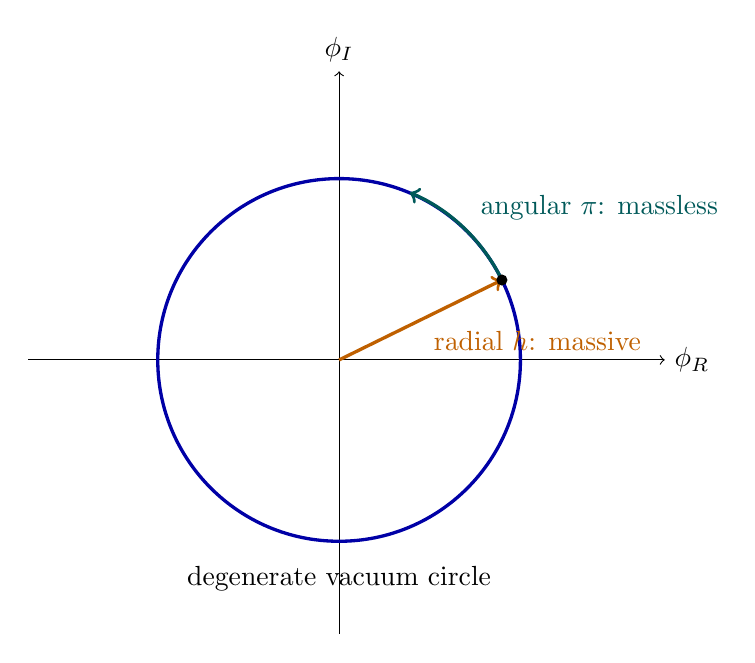
\begin{tikzpicture}[x=0.94cm,y=0.94cm]
  \draw[->] (-4.2,0) -- (4.4,0) node[right] {\(\phi_R\)};
  \draw[->] (0,-3.7) -- (0,3.9) node[above] {\(\phi_I\)};
  \draw[very thick,blue!65!black] (0,0) circle (2.45);
  \draw[->,very thick,orange!75!black] (0,0) -- (2.2,1.08);
  \draw[->,very thick,teal!70!black]
    (2.2,1.08) arc[start angle=26,end angle=67,radius=2.45];
  \node[orange!75!black,below right] at (1.15,0.52)
    {radial \(h\): massive};
  \node[teal!70!black,above right] at (1.78,1.76)
    {angular \(\pi\): massless};
  \fill (2.2,1.08) circle (2pt);
  \node[below] at (0,-2.65) {degenerate vacuum circle};
\end{tikzpicture}
\caption{大域的に破れた理論では、真空円に垂直な方向には曲率があるが、それに沿った方向には曲率がない。動径ヒッグスモードは質量をもち、角度ゴールドストーンモードは質量ゼロである。}
\label{fig:l08-radial-angular}
\end{figure}

次を置く。
\begin{equation}
  \phi(x)=\frac{f+h(x)}{\sqrt2}
           e^{i\pi(x)/f}.
  \label{eq:l08-canonical-polar}
\end{equation}
選ばれた真空の近くで、\(h\) は動径変位を測り、\(\pi\) は正準次元をもつ接線変位を測る。式~\eqref{eq:l08-polar-kinetic}への代入は次を与える。
\begin{equation}
  \partial_\mu\phi^*\,\partial^\mu\phi
  =
  \frac12(\partial_\mu h)^2
  +\frac12\left(1+\frac{h}{f}\right)^2
            (\partial_\mu\pi)^2.
  \label{eq:l08-global-expanded}
\end{equation}
式~\eqref{eq:l08-mexican-hat}のポテンシャルは次を与える。
\begin{equation}
  m_h^2=2\lambda f^2,
  \qquad
  m_\pi^2=0.
  \label{eq:l08-global-masses}
\end{equation}
\(m_h\) よりはるかに低いエネルギーでは、動径運動は高くつくので、一時的に \(h=0\) を凍結してよい。残りのラグランジアンは \(\frac12(\partial\pi)^2\) のみを含み、\(\pi^2\) 項を含まない。これがゴールドストンボソンである。\editorialnote{二箇所で、話された説明は名前を逆にして、ゴールドストーンを食べることがヒッグスボソンに質量を与えると言っている。板書の計算と講義の残りの部分は意図された結果を確立している。すなわち、動径曲率はすでにヒッグスモードに質量を与えており、一方ゲージボソンはゴールドストーンモードを獲得して質量をもつようになる。}

\begin{classroomqa}
\audiencequestion{これが標準模型で唯一の自発的対称性の破れか。\lecturetimestamp{00:16:39}}
\lecturerresponse{電弱ヒッグス相は、ここに関係する確立された対称性の破れの機構である。その実際の対称性は \(SU(2)_L\times U(1)_Y\) であり、この単一の \(U(1)\) ではない。またQCDにはカイラル対称性の破れのような追加の真空構造がある。アーベル的例は、ゲージボソンの機構の意図的に簡略化された模型である。}
\end{classroomqa}

\begin{classroomqa}
\audiencequestion{ヒッグスは自分自身を含むすべての粒子に質量を与えるのか。\lecturetimestamp{00:17:11}}
\lecturerresponse{はいともいいえとも言える区別がある。電弱対称性は\(W\)、\(Z\)、および標準模型のフェルミオンの裸の質量を禁じている。それらの質量は、ヒッグス場がゼロでない平衡の大きさをとった後に現れる。動径方向のヒッグス質量は、自身のポテンシャルの曲率から生じる。他の仮想的な粒子は、この機構とは無関係な、対称性によって許される質量をもちうる。}
\end{classroomqa}

講義は、そのような対称性によって許される質量を、潜在的に非常に重く観測が困難な粒子と結びつけ、可能な例として暗黒物質に言及している。それは動機づけであって、質量の予言ではない。
\editorialnote{暗黒物質の質量スケールは依然として不明である。陽子質量のおよそ千倍の粒子という講義の示唆は歴史的な推測であり、暗黒物質の実験的に確立された性質ではない。}

\begin{classroomqa}
\audiencequestion{\(\rho\)は物理的な半径なのか、それとも場の値なのか。正確には何が動径対称なのか。\lecturetimestamp{00:33:08}}
\lecturerresponse{各時空点において、場の値は補助的な複素平面上の一点であり、\(\rho=|\phi|\)はその点の原点からの距離である。\emph{ポテンシャル}はこの内部平面において動径対称である。すなわち、同じ\(\rho\)をもつすべての点は同じポテンシャルエネルギーをもつ。この半径は通常の空間における距離ではない。}
\end{classroomqa}

\begin{classroomqa}
\audiencequestion{十分に激しい動径方向のキックが、場を中心の極大を越えてポテンシャルの反対側へ運びうるか。
\lecturetimestamp{00:36:00}}
\lecturerresponse{原理的には、十分なエネルギーをもつ局所的な配置は障壁を越えることができる。一様な巨視的場をそれ越しに動かすには莫大なエネルギーが必要であり、一般的な激しい擾乱は、反対側の点にコヒーレントに到達するのではなく、多くの場のモードへエネルギーを放出するであろう。低エネルギー近似が\(\rho\)を凍結するのは、まさにそのような動径方向の励起がそこでは到達不可能だからである。}
\end{classroomqa}

\section{なぜ複素平面は時空ではないのか}

物理的座標と内部的座標の区別は、講義が十分に間を置く価値がある。スカラー場がスカラーと呼ばれるのは、それが物理的な座標軸の回転の下で不変だからである。二つの実スカラー場\(\phi_R(x)\)と\(\phi_I(x)\)は、それらの回転の下で二つのスカラーのままでいる。それらを一つの複素数にまとめることはできるが、この帳簿づけはそれらを空間的ベクトルの成分に変えるものではない。

大域的\(U(1)\)変換は場の\emph{値}を回転させる：
\begin{equation}
\begin{aligned}
  \phi(x)&\longmapsto e^{i\theta}\phi(x),
  \\
  \rho(x)&\longmapsto\rho(x),
  \\
  \alpha(x)&\longmapsto\alpha(x)+\theta.
\end{aligned}
  \label{eq:l08-global-shift}
\end{equation}
同じ定数\(\theta\)がすべての時空点で用いられる。したがって、\(\partial_\mu\alpha\)は変わらない。これはポテンシャルと通常の運動項の両方の対称性である。\(\theta\)が\(x\)に依存することを許すと、微分がその変化を検出し、偏角が変化する。

\section{位相回転を局所化する}

\subsection{通常の微分は失敗する}

次を置く：
\begin{equation}
  \phi'(x)=e^{i\theta(x)}\phi(x).
  \label{eq:l08-local-phase}
\end{equation}
すると
\begin{equation}
  \partial_\mu\phi'
  =e^{i\theta}
    \left(\partial_\mu\phi+i\,\partial_\mu\theta\,\phi\right).
  \label{eq:l08-ordinary-derivative-fails}
\end{equation}
\(\partial_\mu\theta\)に比例する余分な項が、\(\partial_\mu\phi\)が\(\phi\)のように変換するのを妨げる。したがって、\(\partial_\mu\phi^*\partial^\mu\phi\)は任意の局所位相回転の下で不変ではない。

\begin{figure}[htbp]
\centering
\includegraphics[width=0.78\textwidth]{lecture_08_figure_04.png}
\caption{黒板には、局所位相変換と、通常の微分子項が不変に留まることの失敗が記録されている。}
\lectureframe{00:46:49}
\label{fig:l08-local-not-symmetry}
\end{figure}

ベクトルポテンシャルを導入し、一つの規約を一貫して固定する：
\begin{equation}
  D_\mu=\partial_\mu+i g A_\mu,
  \qquad
  A_\mu'=A_\mu-\frac1g\partial_\mu\theta.
  \label{eq:l08-covariant-convention}
\end{equation}
すると
\begin{align}
  D_\mu'\phi'
  &=
  \left(\partial_\mu+i g A_\mu'\right)
  e^{i\theta}\phi
  \notag\\
  &=
  e^{i\theta}
  \left[
    \partial_\mu\phi+i(\partial_\mu\theta)\phi
    +i g A_\mu\phi-i(\partial_\mu\theta)\phi
  \right]
  \notag\\
  &=e^{i\theta}D_\mu\phi.
  \label{eq:l08-covariant-transform}
\end{align}
不要な項が相殺する。共役微分は
\begin{equation}
  (D_\mu\phi)^*
  =(\partial_\mu-i g A_\mu)\phi^*,
\end{equation}
であり、その逆の位相は積において相殺する
\begin{equation}
  (D_\mu\phi)^*D^\mu\phi.
\end{equation}

\begin{classroomqa}
\audiencequestion{前の講義では、ゲージ場の変換は反対の符号で書かれていたか。\lecturetimestamp{00:48:04}}
\lecturerresponse{\(D_\mu\)における符号と変換則における符号を同時に反転させることは、単なる規約である。
\(D_\mu=\partial_\mu+i gA_\mu\)および
\(\phi'=e^{i\theta}\phi\)とすると、整合性は
\(A_\mu'=A_\mu-g^{-1}\partial_\mu\theta\)を要求する。代替の規約も、すべての符号を一緒に変えるならば、同様にうまく機能する。}
\end{classroomqa}

\begin{classroomqa}
\audiencequestion{黒板上で\(\phi\)の大文字形または小文字形を用いることは、異なる場を表すのか。\lecturetimestamp{00:55:02}}
\lecturerresponse{いかなる区別も意図されていない。文字の形が変わるのは手書きであって、追加の操作や第二のスカラーではない。意味のある区別は、プライム、複素共役の星、および時空指数である。}
\end{classroomqa}

\begin{classroomqa}
\audiencequestion{複素共役は、運動項においてローレンツ指数を上げ下げする操作と同じものですか。
\lecturetimestamp{00:56:50}}
\lecturerresponse{いいえ。スターは内部複素場を共役にする。ローレンツ指数は時空計量で上げる：
\(D^\mu=g^{\mu\nu}D_\nu\)。ローレンツスカラーには縮約\((D_\mu\phi)^*D^\mu\phi\)が必要であり、両方の操作が存在し、異なる役割を果たしている。}
\end{classroomqa}

\subsection{ゲージ場は独自の力学を持つ}

場の強さ
\begin{equation}
  F_{\mu\nu}=\partial_\mu A_\nu-\partial_\nu A_\mu
  \label{eq:l08-field-strength}
\end{equation}
は、\(\theta\)の2つの混合二階導関数が相殺するためゲージ不変である。その時間--空間成分は電場を含み、空間--空間成分は磁場を含む。したがって電気力学のスカラー版は
\begin{equation}
  \mathcal L
  =(D_\mu\phi)^*D^\mu\phi
  -V(\phi^*\phi)
  -\frac14F_{\mu\nu}F^{\mu\nu}.
  \label{eq:l08-abelian-higgs}
\end{equation}
である。ここでの荷電場はボソン的である。これはフェルミオンである電子場ではない。荷電ヘリウム原子核やクーパー対凝縮体は、ボソン的荷電自由度がどのように生じうるかを例示している。

対称性の破れの前、ゲージ項は\(A_\mu\)の導関数を含むが、直接の質量項は含まない。
\begin{equation}
  \frac12m_A^2A_\mu A^\mu,
\end{equation}
を加えようと試みるかもしれないが、式~\eqref{eq:l08-covariant-convention}の下で
\begin{equation}
  A_\mu A^\mu
  \longmapsto
  \left(A_\mu-\frac1g\partial_\mu\theta\right)
  \left(A^\mu-\frac1g\partial^\mu\theta\right),
  \label{eq:l08-bare-mass-fails}
\end{equation}
となり、これは\(A_\mu A^\mu\)に等しくない。裸のゲージボソン質量は局所対称性によって禁じられている。

\begin{figure}[htbp]
\centering
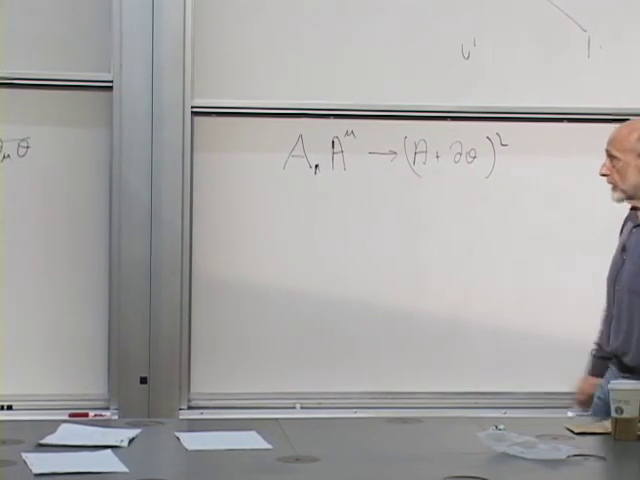
\includegraphics[width=0.76\textwidth]{lecture_08_figure_05.png}
\caption{障害に関する検証済みの板書状態：ゲージ変換の下で、\(A_\mu A^\mu\)は\(\partial_\mu\theta\)を含む平方となるため、裸のベクトル質量は不変ではない。}
\lectureframe{01:07:30}
\label{fig:l08-bare-mass-board}
\end{figure}

\section{ヒッグス機構}

\subsection{共変導関数が質量を生み出す}

破れたポテンシャルに戻り、正準規格化されたパラメトリーゼーション
\begin{equation}
  \phi(x)=\frac{f+h(x)}{\sqrt2}
  e^{i\pi(x)/f}.
\end{equation}
を用いる。その共変導関数は
\begin{equation}
  D_\mu\phi
  =
  \frac{e^{i\pi/f}}{\sqrt2}
  \left[
    \partial_\mu h
    +i(f+h)
      \left(\frac{\partial_\mu\pi}{f}+gA_\mu\right)
  \right].
  \label{eq:l08-covariant-polar}
\end{equation}
である。したがって、
\begin{equation}
\begin{aligned}
  (D_\mu\phi)^*D^\mu\phi
  ={}&
  \frac12(\partial_\mu h)^2
  \\
  &+\frac12(f+h)^2
    \left(\frac{\partial_\mu\pi}{f}+gA_\mu\right)
  \\
  &\hspace{4.2em}\times
    \left(\frac{\partial^\mu\pi}{f}+gA^\mu\right).
\end{aligned}
  \label{eq:l08-higgs-kinetic}
\end{equation}

決定的な項はゲージ選択の前に現れる：
\begin{equation}
  \frac12g^2f^2 A_\mu A^\mu.
  \label{eq:l08-vector-mass-term}
\end{equation}
これをプロカ形式
\(\frac12m_A^2A_\mu A^\mu\)
と比較すると、
\begin{equation}
  \boxed{m_A=g f}.
  \label{eq:l08-vector-mass}
\end{equation}
が得られる。同じ展開は相互作用
\(g^2fh A_\mu A^\mu\)および
\(\frac12g^2h^2A_\mu A^\mu\)も生み出す。したがってベクトル質量は、ゲージ対称性の恣意的な破れではない。それは、非零の平衡振幅\(f\)を持つ相において評価された、ゲージ不変なスカラー運動項から生じる。

\begin{figure}[htbp]
\centering
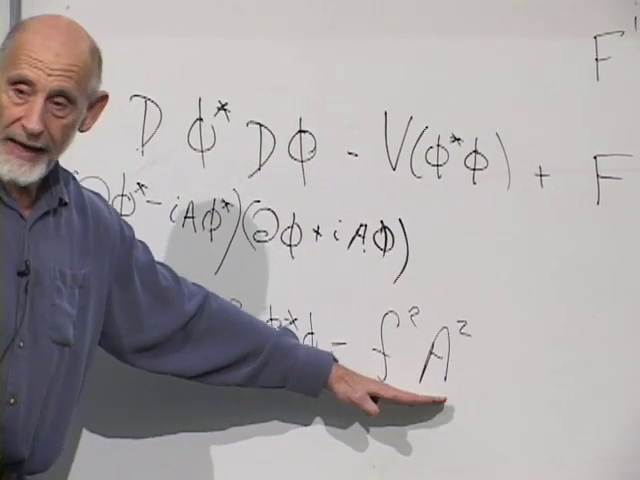
\includegraphics[width=0.78\textwidth]{lecture_08_figure_06.png}
\caption{板書は\((D\phi)^*(D\phi)\)内の\(f^2A^2\)寄与を分離している。数値因子はスカラー場とゲージ結合がどのように規格化されるかに依存する；式~\eqref{eq:l08-canonical-polar}および\eqref{eq:l08-covariant-convention}では、結果は\(m_A=gf\)である。}
\lectureframe{01:10:10}
\label{fig:l08-generated-mass-board}
\end{figure}

講義は\(g\)および\(\sqrt2\)のいくつかの因子を板書表記に吸収しているため、質量を同定する際に\(f\)、\(2f\)、\(\sqrt2f\)の間を一時的に行き来する。これらの因子は、運動項とポテンシャルの規格化が述べられるまで不変な意味を持たない。頑健な結果は\(m_A\propto gf\)であり、式~\eqref{eq:l08-vector-mass}がここで用いられた規約に対する因子を与える。

\subsection{位相は吸収される}

ゲージ変換の下で位相変数は
\begin{equation}
  \pi'(x)=\pi(x)+f\,\theta(x).
\end{equation}
と変化する。
\begin{equation}
  \theta(x)=-\frac{\pi(x)}{f}.
  \label{eq:l08-unitary-gauge-choice}
\end{equation}
を選ぶ。すると\(\pi'=0\)となる。これがユニタリーゲージであり、そこでは
\begin{equation}
  \phi'(x)=\frac{f+h(x)}{\sqrt2}
\end{equation}
が実であり、式~\eqref{eq:l08-higgs-kinetic}は
\begin{equation}
  (D_\mu\phi')^*D^\mu\phi'
  =
  \frac12(\partial_\mu h)^2
  +\frac12g^2(f+h)^2A_\mu'A^{\prime\mu}.
  \label{eq:l08-unitary-gauge-lagrangian}
\end{equation}
に帰着する。角度方向のゴールドストーン場は独立変数のリストから消えたが、ベクトル質量は残っている。

講義はまずこれを低エネルギー極限\(\rho=f\)で示す。そこでは
\begin{align}
  \phi&=f e^{i\alpha},
  \notag\\
  D_\mu\phi
  &=if e^{i\alpha}
    \left(\partial_\mu\alpha+gA_\mu\right),
  \notag\\
  (D_\mu\phi)^*
  &=-if e^{-i\alpha}
    \left(\partial_\mu\alpha+gA_\mu\right).
  \label{eq:l08-frozen-radius}
\end{align}
であり、その積は
\begin{equation}
  f^2
  \left(\partial_\mu\alpha+gA_\mu\right)
  \left(\partial^\mu\alpha+gA^\mu\right).
\end{equation}
である。\(\theta=-\alpha\)を選ぶと\(g^2f^2A_\mu'A^{\prime\mu}\)が残る。

\begin{figure}[htbp]
\centering
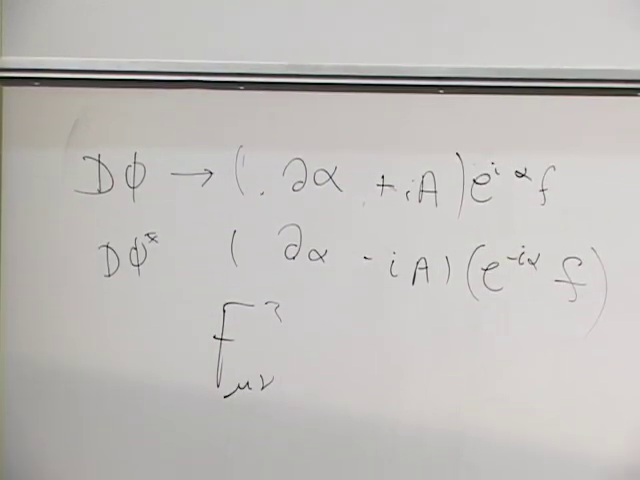
\includegraphics[width=0.82\textwidth]{lecture_08_figure_07.png}
\caption{完全な凍結半径の板書状態：共変導関数は位相導関数とベクトルポテンシャルを一緒に含む。講義は次に\(\theta=-\alpha\)を選び、位相を消去してベクトル質量項を残す。}
\lectureframe{01:16:20}
\label{fig:l08-frozen-radius-board}
\end{figure}

\begin{classroomqa}
\audiencequestion{角度モードの消失を明示する変数でラグランジアン全体を書き直すことはできますか。
\lecturetimestamp{01:13:49}}
\lecturerresponse{はい。極座標変数では、位相はゲージ不変な組み合わせ
\(\partial_\mu\alpha+gA_\mu\)
を通してのみ現れる。\(\theta=-\alpha\)によるゲージ変換は、このゲージが well-defined であるすべての場所で位相をゼロに設定する。するとスカラー運動項はベクトル質量項になり、ゲージ不変な場の強さの項は変わらない。}
\end{classroomqa}

\begin{classroomqa}
\audiencequestion{\(\alpha\)の振動はゲージ振動と区別できませんか。\lecturetimestamp{01:18:02}}
\lecturerresponse{ゲージ理論では、\(\alpha\)の純粋な変化が\(A_\mu\)の対応する変化によって補償される場合、それはゲージ再記述であり、別個の物理的波ではない。不変量は
\(\partial_\mu\alpha+gA_\mu\)
である。大域ゴールドストーン場によって表されていた物理的モードは、質量を持つベクトルの縦偏極として再現する。}
\end{classroomqa}

局所ゲージ対称性が自発的に破れていると言うことがよくある。
操作上、この言い回しは有用である。ゲージを選んだ後、スカラー場は非零の真空値を持ち、スペクトルには質量を持つベクトルが含まれる。
しかし厳密には、ゲージ変換は冗長な記述を関係づけるのであって、異なる物理的状態を関係づけるのではない。
\editorialnote{局所ゲージ冗長性は、大域対称性と同じゲージ不変な意味で破れているのではない。正確な言明は、理論がヒッグス相にあるということである。ゲージ固定された摂動論は、その相を非零のスカラー期待値と、それによって生じる質量を持つベクトルスペクトルによって記述する。}

\section{ゴールドストーン自由度はどこへ行ったか}

変数を変えただけで物理的なものが消えることはありえない。ヒッグス相に入る前と後で自由度を数えよう。

以前：
\begin{equation}
  \underbrace{2}_{\text{massless vector}}
  +
  \underbrace{2}_{\text{complex scalar}}
  =4.
\end{equation}
質量のないベクトルは2つの横偏極を持つ。複素スカラーは動径成分と角度成分という2つの実成分を持つ。

以後：
\begin{equation}
  \underbrace{3}_{\text{massive vector}}
  +
  \underbrace{1}_{\text{radial Higgs}}
  =4.
  \label{eq:l08-degree-count}
\end{equation}
質量を持つベクトルは静止させることができる。その静止系では空間方向が特別扱いされないため、3つの偏極状態を持たなければならない。運動しているときは、2つが横偏極で1つが縦偏極である。ゴールドストーンモードはその縦偏極になったのである。

\begin{figure}[htbp]
\centering
\begin{adjustbox}{max width=\linewidth}
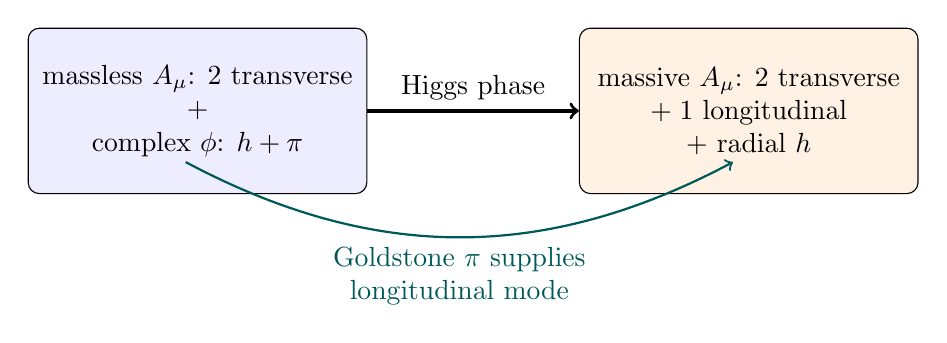
\begin{tikzpicture}[x=1cm,y=1cm]
  \node[draw,rounded corners,fill=blue!7,minimum width=4.3cm,
        minimum height=2.1cm,align=center] (before) at (0,0)
    {massless \(A_\mu\): \(2\) transverse\\
     \(+\)\\
     complex \(\phi\): \(h+\pi\)};
  \node[draw,rounded corners,fill=orange!10,minimum width=4.3cm,
        minimum height=2.1cm,align=center] (after) at (7,0)
    {massive \(A_\mu\): \(2\) transverse\\
     \(+\;1\) longitudinal\\
     \(+\) radial \(h\)};
  \draw[->,very thick] (before) -- node[above]{Higgs phase} (after);
  \draw[->,teal!70!black,thick]
    (-0.15,-0.65) to[bend right=28]
    node[below,align=center]{Goldstone \(\pi\) supplies\\longitudinal mode}
    (6.8,-0.65);
\end{tikzpicture}
\end{adjustbox}
\caption{ヒッグス機構は物理的自由度を破壊するのではなく、再編成する。}
\label{fig:l08-degree-rearrangement}
\end{figure}

\begin{classroomqa}
\audiencequestion{自由度の数え上げを破ることなく、角度自由度がどのように消えることができるのか。\lecturetimestamp{01:19:13}}
\lecturerresponse{物理的には消えない。質量のないベクトルは静止させることができないため、2つのヘリシティを持つ。質量を持つベクトルは縦偏極を含む3つの偏極を持つ。ゴールドストーンモードはその第3の偏極になり、総数は変わらない。}
\end{classroomqa}

この講義は有用な運動学的テストを提供する。質量を持つベクトル粒子を想像し、それを静止するまで減速させ、新しい方向に加速する。もとの運動に対して横偏極であった偏極が、新しい運動に対して縦偏極になりうる。同様に、円偏光した質量を持つ粒子を静止状態を経て反対方向に送ると、そのヘリシティのラベルは反転する。厳密に質量のない粒子はこの実験を通すことができない。どの慣性系でもそれを静止させることはできないからである。したがってその2つのヘリシティは整合的な物理スペクトルをなす。

\section{超伝導との類似}

従来の超伝導体では、電子がクーパー対を形成する。対は電荷\(2e\)を運ぶボソンであり、凝縮体は電荷を持つ複素秩序変数によって記述される。その大きさが非零であるとき、その位相と電磁ベクトルポテンシャルの組み合わせがアンダーソン--ヒッグス機構を生み出す。静磁場はバルク中を自由に伸びるのではなく、ロンドン侵入長の尺度で減衰する。この正確に媒質に依存する意味で、光子は質量を獲得したかのように振る舞う。

この例は冒頭の区別も明らかにする。電磁場が恒久的に別の素粒子に変換されるのではない。質量を持つ伝播則は物質内部の集団状態に属し、外部では真空の光子は質量のないままである。

\section{確立されたこと}

この議論は論理を失うことなく、ここで圧縮できる：
\begin{enumerate}
  \item 破れた大域連続対称性は平坦な角度方向を持ち、したがって質量のないゴールドストーンモードを持つ。
  \item 局所位相不変性はゲージポテンシャルを要求し、\(\partial_\mu\)を\(D_\mu\)に置き換える。
  \item 裸の\(A_\mu A^\mu\)質量は局所変換則を破る。
  \item 電荷を持つスカラーが非零の平衡値\(f\)を持つとき、ゲージ不変な項\(|D_\mu\phi|^2\)は\(\frac12g^2f^2A_\mu A^\mu\)を含む。
  \item 位相はゲージ選択によって除去でき、その物理的自由度は質量を持つベクトルの縦偏極になる。
  \item 動径方向のヒッグス励起は残り、その質量はスカラーポテンシャルの曲率によって決まる。
\end{enumerate}

次の課題はフェルミオンに質量を与えることである。電子とクォークはベクトル機構を直接使うことができない。それらのヒッグス結合は湯川相互作用である。スカラーが\(f\)に落ち着くと、それらの相互作用はフェルミオン質量項になる。

身近な粒子が電弱対称性の破れなしには質量をもたないという広い言明には、最後に一つ限定が必要である。素粒子クォークと荷電レプトンの質量、および\(W\)と\(Z\)の質量は、確かにヒッグス期待値とともに消える。しかしながら、陽子と中性子の質量の大部分は、クォークのヒッグス質量ではなく、QCDの閉じ込めと強場のエネルギーから力学的に生じる。この区別はここで導かれたヒッグス機構を変えるものではない。それはヒッグス機構の適用範囲を精密に保つのである。